\section{Dữ liệu 2}
Bộ dữ liệu ghi lại lịch sử về những ngôi nhà được bán từ 5/2014 đến 5/2015 ở quận King, bang Washington, Hoa Kỳ. Bộ dữ liệu bao gồm 21613 quan trắc, gồm 21 biến.

$*$ \textbf{Phương pháp chọn: Stepwise - lùi; tiêu chuẩn chọn: BIC}.

\subsection*{Tìm hiểu dữ liệu}
%một vài quan trắc đầu tiên, bảng correlation, quan sát phân bố biến Y
\begin{figure}[H]
\centering
\subfloat[Một số quan trắc đầu tiên]
{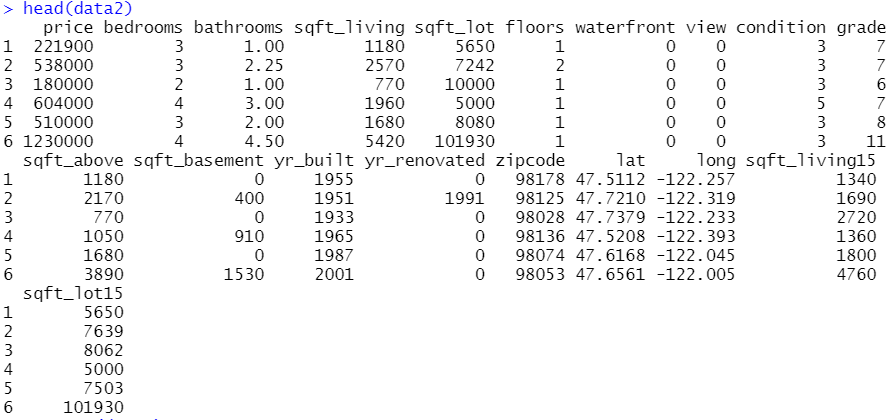
\includegraphics[width=0.7\linewidth]{../Photo Of Result/B2_headdata}}\\
\subfloat[Hệ số tương quan giữa các biến]	{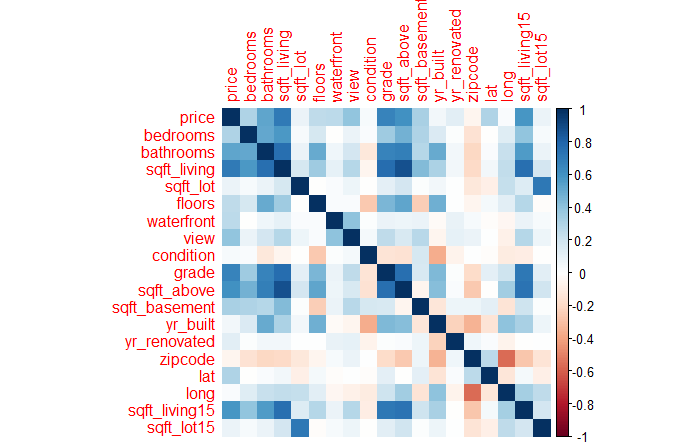
\includegraphics[width=.5\linewidth]{../Photo Of Result/B2_corr}}\hfill
\subfloat[Phân bố của biến phụ thuộc]
{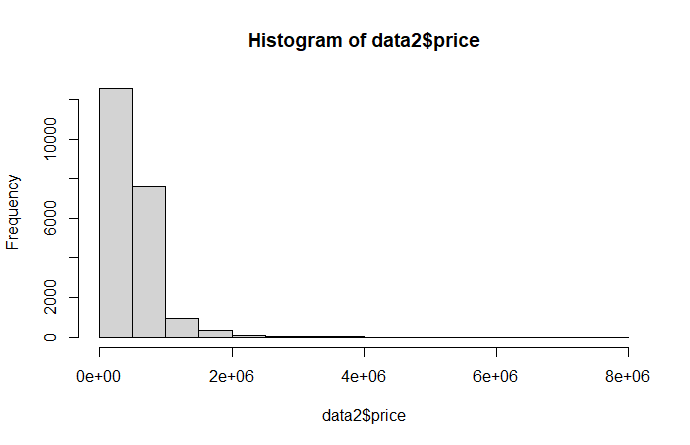
\includegraphics[width=.5\linewidth]{../Photo Of Result/B2_histPrice}}\hfill
\caption{Một số quan sát ban đầu của bộ dữ liệu}
\end{figure}

Bộ dữ liệu cung cấp gồm 21 biến, trong đó biến \texttt{id} và \texttt{date} được loại bỏ khỏi dữ~liệu trước khi tiến hành phân tích, vì nhóm em nghĩ các biến này chỉ để ghi lại chỉ số và thời gian mua bán, không mang nhiều ý nghĩa thống kê. 

Quan sát ban đầu cho thấy: các biến độc lập \texttt{bathrooms} (số phòng tắm), \texttt{sqft\_living} (diện tích căn nhà), \texttt{grade} (điểm số đánh giá), \texttt{sqft\_above} (diện tích ngoài tầng hầm), \texttt{sqft\_living15} (diện tích ngôi nhà vào năm 2015) có mối tương quan cao với biến phụ~thuộc \texttt{Price} - giá nhà; biến phụ thuộc \texttt{Price} phân bố không đều, bị lệch hẳn về một~phía và giá trị chủ yếu từ 0 đến 2 000 000.
\subsection*{Phân tích, chọn mô hình}
%mô hình ban đầu (Đầy đủ biến, chưa chuẩn hóa), mô hình sau khi chọn biến bằng các tiêu chuẩn ..., mô hình cuối cùng (nếu có chuẩn hóa dữ liệu)

%đưa ra kết quả R của mỗi mô hình, giải thích vì sao chọn mô hình cuối cùng, phân tích các kết quả từ plot xem mô hình có đảm bảo các giả thiết hay không (kỳ vọng = 0, phân phối chuẩn, phương sai không đổi, có mối quan hệ tuyến tính, không có đa cộng tuyến)
\begin{figure}[H]
	\centering
	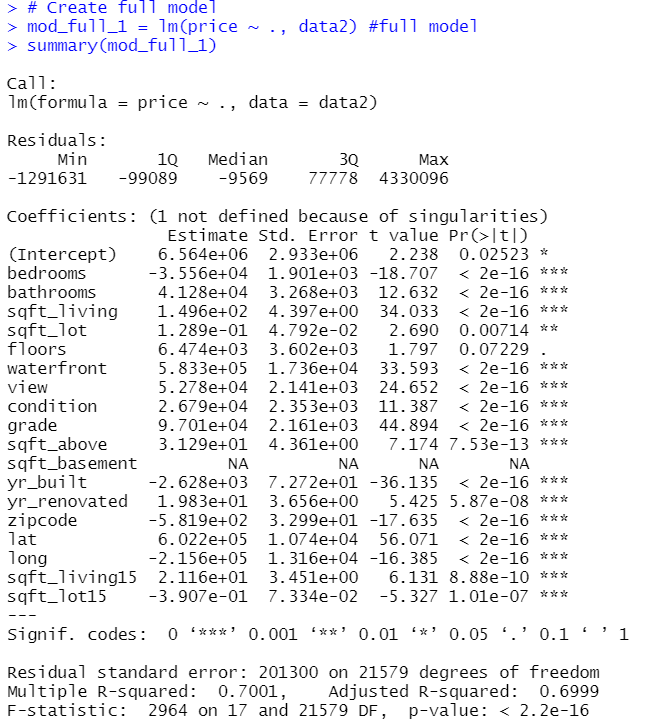
\includegraphics[width=.7\linewidth]{../Photo Of Result/B2_originalmodel_R}
	\caption{Mô hình hồi quy đầy đủ ban đầu}
	\label{B2_full}
\end{figure}

Bộ dữ liệu (sau khi loại bỏ \texttt{id} và \texttt{date}) có 18 biến giải thích, do đó nhóm em chọn phương pháp lùi (\textbf{stepwise - backward}) cho bộ dữ liệu này. Trong mô hình hồi quy đầy đủ (Hình \ref{B2_full}), đa số các biến giải thích đều có ý nghĩa thống kê, do đó tiến hành phương~pháp lùi (loại biến dần dần) sẽ tiết kiệm thời gian hơn so với các phương pháp còn lại.  Tiêu chuẩn BIC có xu hướng chọn các mô hình ít phức tạp hơn so với tiêu chuẩn AIC, đặc biệt khi số lượng quan trắc lớn.

\begin{figure}[H]
	\centering
	\subfloat[Chọn biến]
	{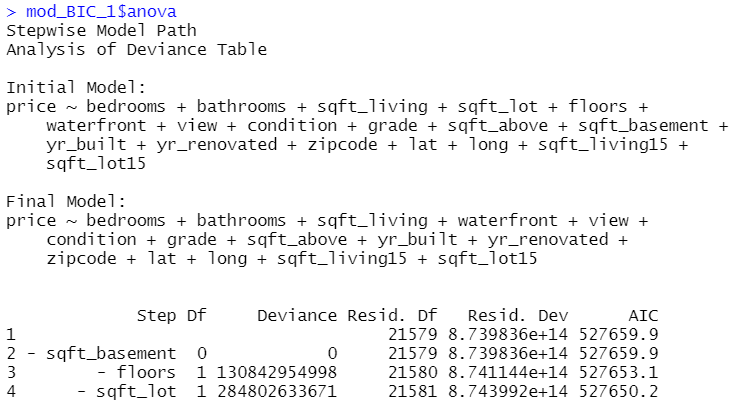
\includegraphics[width=.5\linewidth]{../Photo Of Result/B2_BIC}}\hfill
	\subfloat[Kết quả mô hình]
	{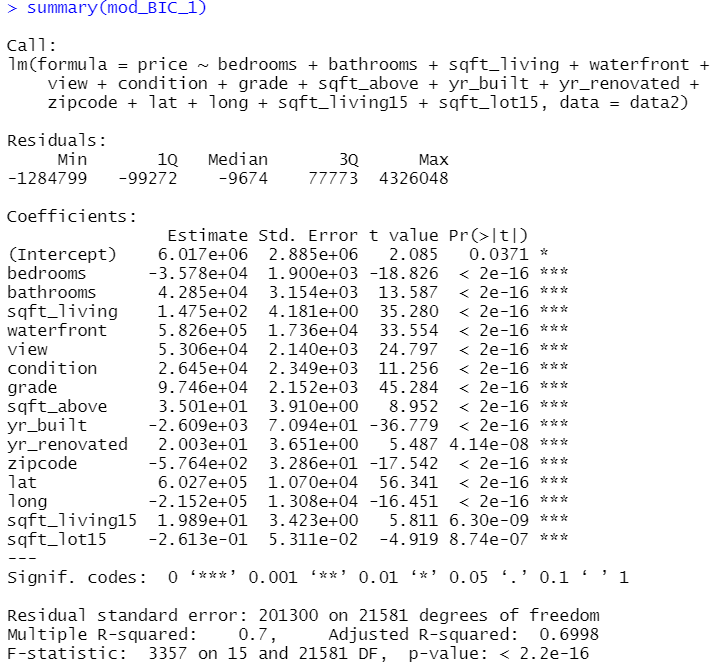
\includegraphics[width=.5\linewidth]{../Photo Of Result/B2_modBIC1_R}}
	\caption{Mô hình khi chọn bằng tiêu chuẩn BIC}
	\label{B2_BIC}
\end{figure}
 Bằng phương pháp lùi và tiêu chuẩn BIC (Hình \ref{B2_BIC}), các biến \texttt{sqft\_basement, floors, sqft\_lot} đã bị loại bỏ khỏi mô hình. Mô hình được chọn có $R^2=0.7$, $R^2_{adj}=0.69$, các tham số ước lượng của mô hình đều có ý nghĩa thống kê.
 
 Ta tiến hành kiểm tra xem mô hình này có thỏa mãn các giả thiết của mô hình hồi~quy hay không.
 
 \begin{figure}[H]
 	\centering
 	{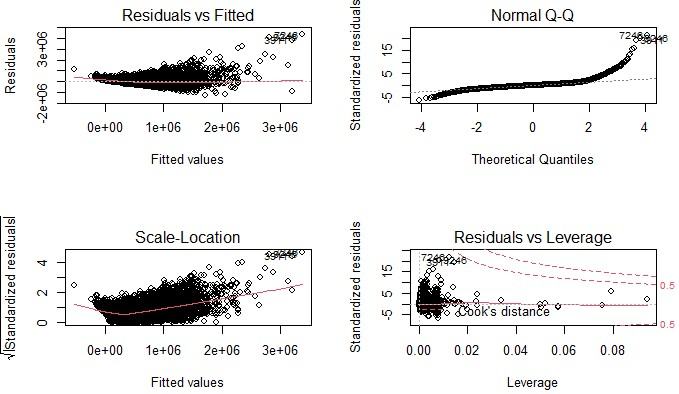
\includegraphics[width=.7\linewidth]{../Photo Of Result/B2_originalmodel}}
 	\caption{Các biểu đồ kiểm định mô hình}
 	\label{B2_check}
 \end{figure}
 
 Dựa vào hình \ref{B2_check}, phương sai của sai số không phải là hằng số, kì vọng của sai số bằng 0; sai số có vẻ tuân theo phân phối chuẩn nhưng phần đuôi trên bị lệch khá nhiều. 
 
 Kết hợp với nhận xét ban đầu, về việc biến \texttt{Price} phân bố không đều, nhóm em tiến~hành biến đổi biến này thành \texttt{log(Price)}.
 
 \begin{figure}[H]
 	\centering
 	{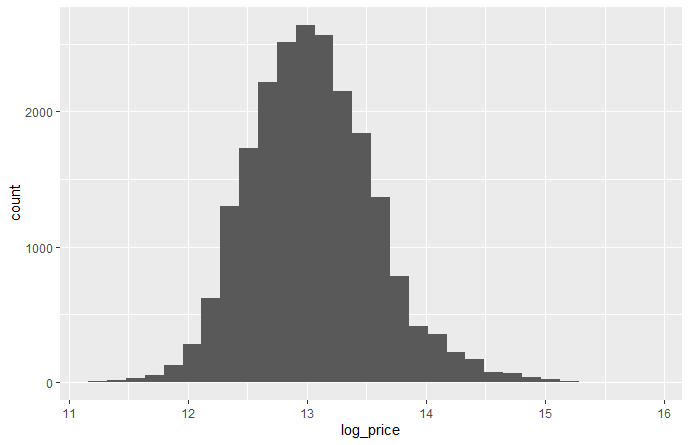
\includegraphics[width=.5\linewidth]{../Photo Of Result/B2_logprice}}
 	\caption{Phân bố của biến \texttt{Price} sau khi biến đổi }
 	\label{B2_log}
 \end{figure}
 Sau khi biến đổi, ta tiến hành hồi quy cho: \textbf{mô hình 1} mô hình có 15 biến đã chọn bằng tiêu chuẩn BIC trước đó, và \textbf{mô hình 2} mô hình đầy đủ rồi áp dụng tiêu chuẩn BIC để chọn biến.
 
  \begin{figure}[H]
 	\centering
 	\subfloat[Mô hình 1]
 	{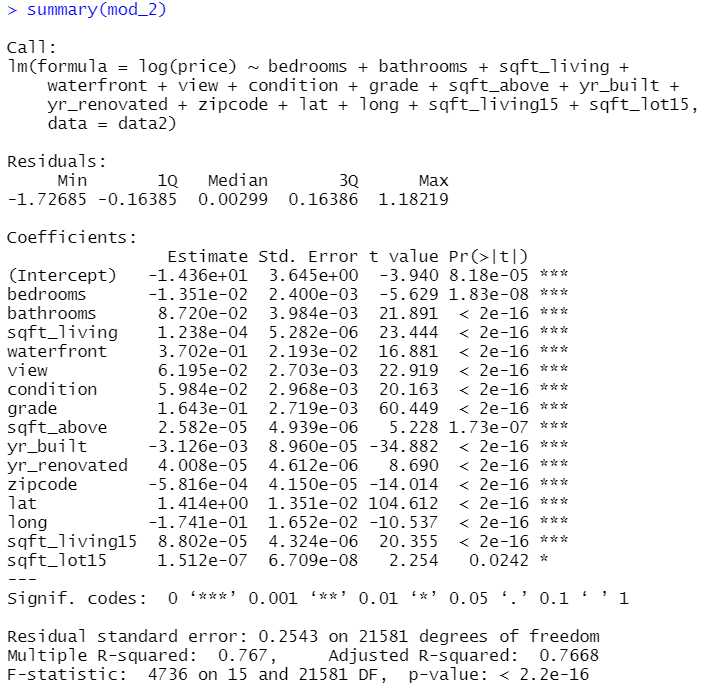
\includegraphics[width=.5\linewidth]{../Photo Of Result/B2_log}}\hfill
 	\subfloat[Mô hình 2]
 	{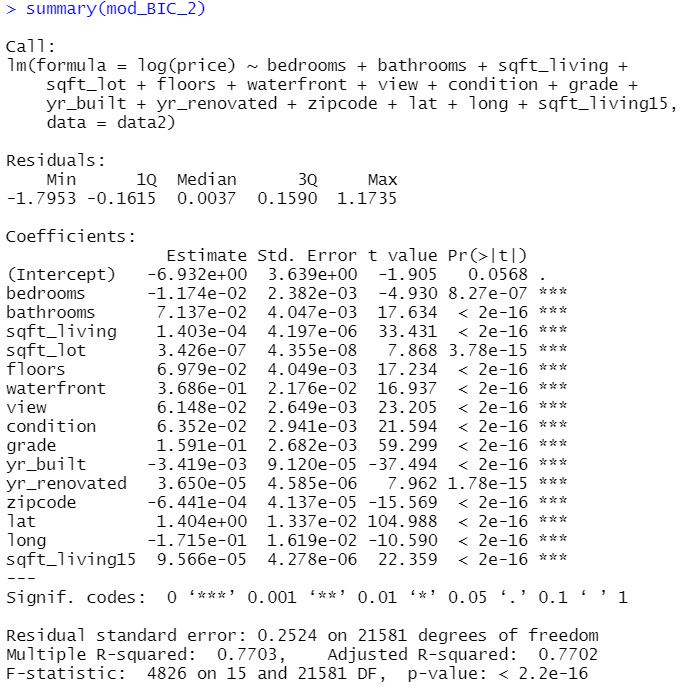
\includegraphics[width=.48\linewidth]{../Photo Of Result/B2_modBIC2_R}}
 	\caption{Kết quả khi biến đổi \texttt{Price} thành \texttt{log(Price)}}
 \end{figure}
 
Cả hai mô hình đều gồm 15 biến giải thích, mô hình 2 đã loại bỏ các biến \texttt{sqft\_basement, sqft\_above, sqft\_lot15} khác với 3 biến đã loại trước khi biến đổi \texttt{Price}. 

Nhóm em chọn \textbf{mô hình 2} là mô hình cuối cùng, vì: mô hình 2 có hệ số xác định lớn hơn ($R^2=77.03\%$), các biến liên quan đến diện tích tầng hầm (\texttt{sqft\_basement}, \texttt{sqft\_above}) đã được bao gồm trong \texttt{sqft\_living}, diện tích khu đất vào năm 2015 cũng không mang nhiều ý nghĩa thống kê trong mô hình 1 nên có thể loại bỏ.

\textit{Kiểm tra giả thiết mô hình 2:} phương sai của sai số không thay~đổi, kì vọng bằng 0 và đã tuân theo phân phối chuẩn, chưa phát hiện hiện tượng đa~cộng~tuyến trong mô~hình (các chỉ số VIF $< 5$) (Hình \ref{B2_final}). 

 \begin{figure}[H]
	\centering
	\subfloat[Các biểu đồ kiểm định]
	{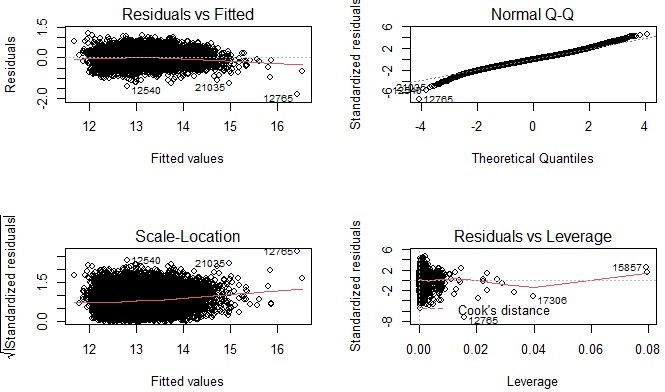
\includegraphics[width=\linewidth]{../Photo Of Result/B2_modBIC2_fitted}}\hfill
	\subfloat[Kiểm tra đa cộng tuyến]
	{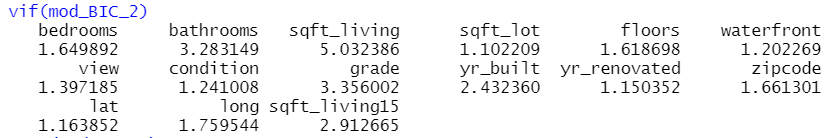
\includegraphics[width=\linewidth]{../Photo Of Result/B2_BIC_vif}}
	\caption{Kết quả khi biến đổi thành \texttt{log(Price)}}
	\label{B2_final}
\end{figure}

Vậy \textbf{mô hình cuối cùng được chọn} có các hệ số ước lượng như hình \ref{B2_coef}.
\begin{figure}[H]
	\centering
	{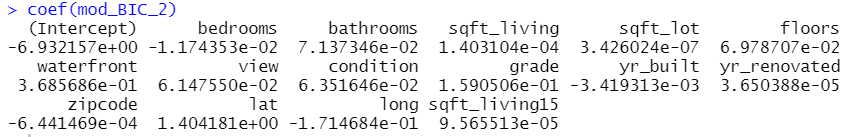
\includegraphics[width=\linewidth]{../Photo Of Result/B2_coef}}
	\caption{Hệ số mô hình được chọn}
	\label{B2_coef}
\end{figure}

\noindent $\log$\texttt{(Price)} = $-6.93 -0.011 \times$ \texttt{bedrooms} $+0.071\times$ \texttt{bathrooms} $+1.403\times 10^{-4} \times$ \texttt{sqft\_living}

\hspace{1.5cm} $+ 3.426\times10^{-7}\times$ \texttt{sqft\_lot} $+ 0.069\times$ \texttt{floors} $+ 0.36\times$ \texttt{waterfront} $+ 0.061\times$ \texttt{view}

\hspace{1.5cm}  $+ 0.063\times$ \texttt{condition} $+ 0.159\times$ \texttt{grade} $- 3.4196\times 10^{-3}\times$ \texttt{yr\_built}

\hspace{1.5cm} $+ 3.650\times 10^{-5}\times$ \texttt{yr\_renovated} $- 6.441 \times 10^{-4}\times$ \texttt{zipcode} $+ 1.404\times$ \texttt{lat}


\hspace{1.5cm}  $- 0.171\times$ \texttt{long} $+ 9.565.171\times 10^{-5}\times$ \texttt{sqft\_living15}

\subsection*{Kết luận}
%Nhận xét các biến ảnh hưởng đến biến Y từ mô hình cuối cùng, ý nghĩa của mô hình đã chọn

Có 77.06\% sự biến thiên của giá nhà ở quận King được giải thích bởi 15 biến độc~lập, trong đó các yếu tố ảnh hưởng nhiều nhất gồm \textit{số phòng ngủ, số phòng tắm, diện~tích~nhà, số tầng, hướng nhà ra bờ sông, tình trạng ngôi nhà (mới/cũ), điểm theo phân loại của quận, vị trí (kinh độ - vĩ độ), năm xây dựng}.

Giá trị của một căn nhà \textbf{không bị ảnh hưởng nhiều} bởi các yếu tố: diện tích tầng~hầm, diện tích khu đất, diện tích ngoài tầng hầm, năm sửa chữa căn nhà, zipcode (mã~vùng) của ngôi nhà. Diện tích của căn nhà cũng có ảnh hưởng, tuy nhiên sự ảnh~hưởng là không nhiều.

Số phòng ngủ có mối tương quan nghịch với giá nhà, vì khi số phòng ngủ tăng lên, nhưng các yếu tố còn lại không thay đổi, thì diện tích của mỗi phòng ngủ sẽ giảm đi, gây cảm giác chật chội. 

Nhìn vào các kết quả hình \ref{B2_final}, vẫn thấy có nhiều điểm ngoại lai (\textbf{outlier}), hướng~nghiên cứu tiếp theo có thể loại bỏ những điểm này ra khỏi bộ dữ liệu, tiến~hành quan~sát riêng để rút ra thêm các kết luận khác (nếu có).